\subsection{直线}\label{subsec:czjh1-1-1}

在小学里我们学过\zhongdian{直线}。 一根拉紧的线、一张纸的折痕都给我们以直线的形象。
直线是向两方无限延伸着的。

一条直线上有无限多个点。 点可以用一个大写字母来表示。
如图 \ref{fig:czjh1-1-1} 中的点, 记作点 $A$、点 $B$、点 $C$、…。
直线可以用表示它上面任意两个点的大写字母来表示,也可以用一个小写字母来表示。
如图 \ref{fig:czjh1-1-1} 中的直线可以记作直线 $AB$, 也可以记作直线 $l$。


\begin{figure}[htbp]
    \centering
    \begin{minipage}[b]{4cm}
        \centering
        % 使用 tkz-euclide 绘图的代码
\begin{tikzpicture}
	\tkzDefPoints{-0.7/0/M, 0/0/A, 0.7/0/N, 1/0/B, 1.5/0/C}
	\tkzDrawLine[add=0.8 and 0.5](A,C)
	\tkzLabelLine[pos=1.5,right](A,C){$l$}
	\tkzDrawPoints[fill=black](A,B,C,M,N)
	\tkzLabelPoints[above](A,B,C)
\end{tikzpicture}

% 下面是直接使用 tikz 绘图的代码,放在这里作对比
% \begin{tikzpicture}
% 	\coordinate (A) at (0,0);
% 	\coordinate (B) at (1.0,0);
% 	\coordinate (C) at (1.5,0);
% 	\coordinate (M) at (-0.7,0);
% 	\coordinate (N) at ( 0.7,0);

% 	\draw (-1.2,0) -- (2.25, 0) node[right] {$l$}; % AC长 1.5, 1.5+1.5*0.5=2.25;  1.5*0.8=1.2
% 	\foreach \x in {A,B,C,M,N} {
% 		\draw[fill=black] (\x) circle (1pt);
% 	}
% 	\foreach \x in {A,B,C} {
% 		\draw (\x) node [above] {$\x$};
% 	}
% \end{tikzpicture}


        \caption{}\label{fig:czjh1-1-1}
    \end{minipage}
    \qquad
    \begin{minipage}[b]{4cm}
        \centering
        \begin{tikzpicture}
	\tkzDefPoints{0/0/A, 0/1/a, 1/0.3/b, 1.2/-0.5/c, 0.8/0.8/d}
	\tkzDrawLines[add=1 and 0](A,a  A,b  A,c  A,d)
	\tkzLabelLine[pos=1,above](A,a){$a$}
	\tkzLabelLine[pos=1,right](A,b){$b$}
	\tkzLabelLine[pos=1,right](A,c){$c$}
	\tkzDrawPoint(A)
	\tkzLabelPoints[below right, yshift=-0.3em](A)
\end{tikzpicture}


        \caption{}\label{fig:czjh1-1-2}
    \end{minipage}
    \qquad
    \begin{minipage}[b]{4cm}
        \centering
        \begin{tikzpicture}
	\tkzDefPoints{0/0/A, 1/0/B}
	\tkzDrawLine[add=0.7 and 0.7](A,B)
	\tkzDrawPoints[fill=black](A,B)
	\tkzLabelPoints[above](A,B)
\end{tikzpicture}


        \caption{}\label{fig:czjh1-1-3}
    \end{minipage}
\end{figure}

画直线可以用直尺,把直尺放在纸上或黑板上,用笔沿着直尺的边缘就可以画出一条直线,
但画出的只是直线的一部分。

如图 \ref{fig:czjh1-1-2} 那样,经过一点 $A$ 可以画出任意多条直线 $a$、$b$、$c$、…。
也就是说,经过一点的直线有无数条。

如果我们经过两点来画直线,如图 \ref{fig:czjh1-1-3} 那样,经过点 $A$ 与点 $B$ 只能画出一条直线来。
人们总结了这一经验,得到直线的基本性质:

\begin{xingzhi}
    经过两点有一条直线,并且只有一条直线。
\end{xingzhi}

这句话可以简单说成:\begin{xingzhi}
    两点确定一条直线。
\end{xingzhi}

在几何里,象这样,人们从实践经验中总结出来的图形的基本性质,我们把它叫做\zhongdian{公理}。
公理可以作为说明其他问题的根据。

在日常生活和生产实践中,经常用到直线的这种性质,
例如,架线工人在立电线杆时,只要定出两根杆的位置(即两个点),
就能定出一行电线杆所在直线的位置,而且只能定出一条这样的直线(图 \ref{fig:czjh1-1-4});
锯木料时,经过刨平的木板上的两个点,就能弹出一条笔直的墨线,而且只能弹出一条这样的墨线(图 \ref{fig:czjh1-1-5})。

\begin{figure}[htbp]
    \centering
    \begin{minipage}[b]{5cm}
        \centering
        \includegraphics[width=3.8cm]{../pic/czjh1-ch1-04.png}
        \caption{}\label{fig:czjh1-1-4}
    \end{minipage}
    \qquad
    \begin{minipage}[b]{5cm}
        \centering
        \includegraphics[width=3.8cm]{../pic/czjh1-ch1-05.png}
        \caption{}\label{fig:czjh1-1-5}
    \end{minipage}
    \qquad
    \begin{minipage}[b]{4cm}
        \centering
        \begin{tikzpicture}
	\tkzDefPoints{2/1/A, 0/0/B,  0/1/C,  2/0/D}
	\tkzInterLL(A,B)(C,D)	\tkzGetPoint{O}
	\tkzDrawSegments(A,B  C,D)
	\tkzLabelPoints[left](B,C)
	\tkzLabelPoints[right](A,D)
	\tkzLabelPoints[above](O)
\end{tikzpicture}


        \caption{}\label{fig:czjh1-1-6}
    \end{minipage}
\end{figure}

在图 \ref{fig:czjh1-1-6} 中,两条直线 $AB$、$CD$ 都经过同一个点 $O$, 我们说这\zhongdian{两条直线相交},
点 $O$ 是这两条直线的\zhongdian{交点}, 说成 “直线 $AB$、 $CD$ 相交于点 $O$”。

根据直线的公理,可以推出下面的性质:

\begin{xingzhi}
    两条直线相交,只有一个交点。
\end{xingzhi}

这是因为,假如两条直线有两个交点,那么,经过两个点有两条直线,
这与 “经过两点只有一条直线” 是不符合的。所以两条直线有两个交点是不可能的。


\begin{lianxi}

\jiange
\begin{minipage}{12cm}

    \xiaoti{已知图中的三个点,它们不在同一条直线上。}

    \begin{xiaoxiaotis}

        \xxt{经过其中每两个点都画一条直线,这样一共可以画几条直线。}

        \xxt{分别用大写字母表示图中的点,并说出每一条直线的名称。}

        \xxt{分别用一个小写字母表示图中的每一条直线,并说明各条直线是由哪两个点确定的。}

    \end{xiaoxiaotis}
\end{minipage}
\quad
\begin{minipage}{3.5cm}
    \centering
    \begin{tikzpicture}
	\tkzDefPoints{0/0/A, 2/-0.3/B,  1/1/C}
	\tkzDrawPoints[fill=black](A, B, C)
\end{tikzpicture}


    (第 1 题)
\end{minipage}\jiange

\xiaoti{读下列语句,并画出它们的图形:}
\begin{xiaoxiaotis}

    \xxt{直线 $AB$ 经过点 $C$ ;}

    \xxt{点 $D$ 在直线 $EF$ 上, 但在直线 $GH$ 外(即点 $D$ 不在直线 $GH$ 上);}

    \xxt{直线 $a$、 $b$ 相交于点 $C$、直线 $b$、 $c$ 相交于点 $A$,
         直线 $a$、 $c$ 相交于点 $B$。这时我们说 “直线 $a$、$b$、$c$ 两两相交”。
    }

\end{xiaoxiaotis}

\end{lianxi}

